\documentclass[]{article}
\usepackage{lmodern}
\usepackage{amssymb,amsmath}
\usepackage{ifxetex,ifluatex}
\usepackage{fixltx2e} % provides \textsubscript
\ifnum 0\ifxetex 1\fi\ifluatex 1\fi=0 % if pdftex
  \usepackage[T1]{fontenc}
  \usepackage[utf8]{inputenc}
\else % if luatex or xelatex
  \ifxetex
    \usepackage{mathspec}
  \else
    \usepackage{fontspec}
  \fi
  \defaultfontfeatures{Ligatures=TeX,Scale=MatchLowercase}
\fi
% use upquote if available, for straight quotes in verbatim environments
\IfFileExists{upquote.sty}{\usepackage{upquote}}{}
% use microtype if available
\IfFileExists{microtype.sty}{%
\usepackage{microtype}
\UseMicrotypeSet[protrusion]{basicmath} % disable protrusion for tt fonts
}{}
\usepackage[margin=1in]{geometry}
\usepackage{hyperref}
\hypersetup{unicode=true,
            pdftitle={Zhang\_HW2},
            pdfborder={0 0 0},
            breaklinks=true}
\urlstyle{same}  % don't use monospace font for urls
\usepackage{color}
\usepackage{fancyvrb}
\newcommand{\VerbBar}{|}
\newcommand{\VERB}{\Verb[commandchars=\\\{\}]}
\DefineVerbatimEnvironment{Highlighting}{Verbatim}{commandchars=\\\{\}}
% Add ',fontsize=\small' for more characters per line
\usepackage{framed}
\definecolor{shadecolor}{RGB}{248,248,248}
\newenvironment{Shaded}{\begin{snugshade}}{\end{snugshade}}
\newcommand{\AlertTok}[1]{\textcolor[rgb]{0.94,0.16,0.16}{#1}}
\newcommand{\AnnotationTok}[1]{\textcolor[rgb]{0.56,0.35,0.01}{\textbf{\textit{#1}}}}
\newcommand{\AttributeTok}[1]{\textcolor[rgb]{0.77,0.63,0.00}{#1}}
\newcommand{\BaseNTok}[1]{\textcolor[rgb]{0.00,0.00,0.81}{#1}}
\newcommand{\BuiltInTok}[1]{#1}
\newcommand{\CharTok}[1]{\textcolor[rgb]{0.31,0.60,0.02}{#1}}
\newcommand{\CommentTok}[1]{\textcolor[rgb]{0.56,0.35,0.01}{\textit{#1}}}
\newcommand{\CommentVarTok}[1]{\textcolor[rgb]{0.56,0.35,0.01}{\textbf{\textit{#1}}}}
\newcommand{\ConstantTok}[1]{\textcolor[rgb]{0.00,0.00,0.00}{#1}}
\newcommand{\ControlFlowTok}[1]{\textcolor[rgb]{0.13,0.29,0.53}{\textbf{#1}}}
\newcommand{\DataTypeTok}[1]{\textcolor[rgb]{0.13,0.29,0.53}{#1}}
\newcommand{\DecValTok}[1]{\textcolor[rgb]{0.00,0.00,0.81}{#1}}
\newcommand{\DocumentationTok}[1]{\textcolor[rgb]{0.56,0.35,0.01}{\textbf{\textit{#1}}}}
\newcommand{\ErrorTok}[1]{\textcolor[rgb]{0.64,0.00,0.00}{\textbf{#1}}}
\newcommand{\ExtensionTok}[1]{#1}
\newcommand{\FloatTok}[1]{\textcolor[rgb]{0.00,0.00,0.81}{#1}}
\newcommand{\FunctionTok}[1]{\textcolor[rgb]{0.00,0.00,0.00}{#1}}
\newcommand{\ImportTok}[1]{#1}
\newcommand{\InformationTok}[1]{\textcolor[rgb]{0.56,0.35,0.01}{\textbf{\textit{#1}}}}
\newcommand{\KeywordTok}[1]{\textcolor[rgb]{0.13,0.29,0.53}{\textbf{#1}}}
\newcommand{\NormalTok}[1]{#1}
\newcommand{\OperatorTok}[1]{\textcolor[rgb]{0.81,0.36,0.00}{\textbf{#1}}}
\newcommand{\OtherTok}[1]{\textcolor[rgb]{0.56,0.35,0.01}{#1}}
\newcommand{\PreprocessorTok}[1]{\textcolor[rgb]{0.56,0.35,0.01}{\textit{#1}}}
\newcommand{\RegionMarkerTok}[1]{#1}
\newcommand{\SpecialCharTok}[1]{\textcolor[rgb]{0.00,0.00,0.00}{#1}}
\newcommand{\SpecialStringTok}[1]{\textcolor[rgb]{0.31,0.60,0.02}{#1}}
\newcommand{\StringTok}[1]{\textcolor[rgb]{0.31,0.60,0.02}{#1}}
\newcommand{\VariableTok}[1]{\textcolor[rgb]{0.00,0.00,0.00}{#1}}
\newcommand{\VerbatimStringTok}[1]{\textcolor[rgb]{0.31,0.60,0.02}{#1}}
\newcommand{\WarningTok}[1]{\textcolor[rgb]{0.56,0.35,0.01}{\textbf{\textit{#1}}}}
\usepackage{graphicx,grffile}
\makeatletter
\def\maxwidth{\ifdim\Gin@nat@width>\linewidth\linewidth\else\Gin@nat@width\fi}
\def\maxheight{\ifdim\Gin@nat@height>\textheight\textheight\else\Gin@nat@height\fi}
\makeatother
% Scale images if necessary, so that they will not overflow the page
% margins by default, and it is still possible to overwrite the defaults
% using explicit options in \includegraphics[width, height, ...]{}
\setkeys{Gin}{width=\maxwidth,height=\maxheight,keepaspectratio}
\IfFileExists{parskip.sty}{%
\usepackage{parskip}
}{% else
\setlength{\parindent}{0pt}
\setlength{\parskip}{6pt plus 2pt minus 1pt}
}
\setlength{\emergencystretch}{3em}  % prevent overfull lines
\providecommand{\tightlist}{%
  \setlength{\itemsep}{0pt}\setlength{\parskip}{0pt}}
\setcounter{secnumdepth}{0}
% Redefines (sub)paragraphs to behave more like sections
\ifx\paragraph\undefined\else
\let\oldparagraph\paragraph
\renewcommand{\paragraph}[1]{\oldparagraph{#1}\mbox{}}
\fi
\ifx\subparagraph\undefined\else
\let\oldsubparagraph\subparagraph
\renewcommand{\subparagraph}[1]{\oldsubparagraph{#1}\mbox{}}
\fi

%%% Use protect on footnotes to avoid problems with footnotes in titles
\let\rmarkdownfootnote\footnote%
\def\footnote{\protect\rmarkdownfootnote}

%%% Change title format to be more compact
\usepackage{titling}

% Create subtitle command for use in maketitle
\newcommand{\subtitle}[1]{
  \posttitle{
    \begin{center}\large#1\end{center}
    }
}

\setlength{\droptitle}{-2em}
  \title{Zhang\_HW2}
  \pretitle{\vspace{\droptitle}\centering\huge}
  \posttitle{\par}
  \author{}
  \preauthor{}\postauthor{}
  \date{}
  \predate{}\postdate{}


\begin{document}
\maketitle

\hypertarget{james-cutler}{%
\section{James Cutler}\label{james-cutler}}

\hypertarget{wk-2-homework-zhang}{%
\section{WK 2 homework Zhang}\label{wk-2-homework-zhang}}

\hypertarget{alsm-1.43-2.2-2.17-2.62}{%
\subsection{ALSM 1.43, 2.2, 2.17, 2.62}\label{alsm-1.43-2.2-2.17-2.62}}

\begin{Shaded}
\begin{Highlighting}[]
\KeywordTok{library}\NormalTok{(ggplot2)}
\end{Highlighting}
\end{Shaded}

\hypertarget{section}{%
\section{1.43}\label{section}}

\begin{Shaded}
\begin{Highlighting}[]
\NormalTok{CDI =}\StringTok{ }\KeywordTok{read.csv}\NormalTok{(}\StringTok{"/Users/jamescutler/Desktop/Biostats_II/APPENC02.csv"}\NormalTok{, }
               \DataTypeTok{header =} \OtherTok{FALSE}\NormalTok{)}
\NormalTok{CDI =}\StringTok{ }\NormalTok{CDI[}\DecValTok{3}\OperatorTok{:}\KeywordTok{ncol}\NormalTok{(CDI)]}
\KeywordTok{colnames}\NormalTok{(CDI) =}\StringTok{ }\KeywordTok{c}\NormalTok{(}\StringTok{"County"}\NormalTok{,}\StringTok{"State"}\NormalTok{,}\StringTok{"S_Area"}\NormalTok{,}\StringTok{"Pop"}\NormalTok{,}\StringTok{"Per18_34"}\NormalTok{,}\StringTok{"Per65up"}\NormalTok{,}\StringTok{"Physicians"}\NormalTok{,}
                  \StringTok{"Hosp_beds"}\NormalTok{,}\StringTok{"Crimes"}\NormalTok{,}\StringTok{"PerHSgrads"}\NormalTok{,}\StringTok{"PerBach"}\NormalTok{,}\StringTok{"PerPoor"}\NormalTok{,}\StringTok{"PerUnemp"}\NormalTok{,}
                  \StringTok{"PerCapInc"}\NormalTok{,}\StringTok{"PersonalInc"}\NormalTok{,}\StringTok{"GeoReg"}\NormalTok{)}
\end{Highlighting}
\end{Shaded}

\hypertarget{plots-in-ggplot2}{%
\section{Plots in ggplot2:}\label{plots-in-ggplot2}}

\begin{Shaded}
\begin{Highlighting}[]
\KeywordTok{ggplot}\NormalTok{(CDI, }\KeywordTok{aes}\NormalTok{(Pop,Physicians)) }\OperatorTok{+}
\StringTok{  }\KeywordTok{geom_point}\NormalTok{(}\DataTypeTok{alpha =} \FloatTok{.1}\NormalTok{, }\DataTypeTok{col =} \StringTok{"red"}\NormalTok{) }\OperatorTok{+}
\StringTok{  }\KeywordTok{geom_smooth}\NormalTok{(}\DataTypeTok{method =} \StringTok{"lm"}\NormalTok{, }\DataTypeTok{se =} \OtherTok{FALSE}\NormalTok{, }\DataTypeTok{size =} \FloatTok{.3}\NormalTok{) }\OperatorTok{+}\StringTok{ }
\StringTok{  }\KeywordTok{theme_bw}\NormalTok{()}
\end{Highlighting}
\end{Shaded}

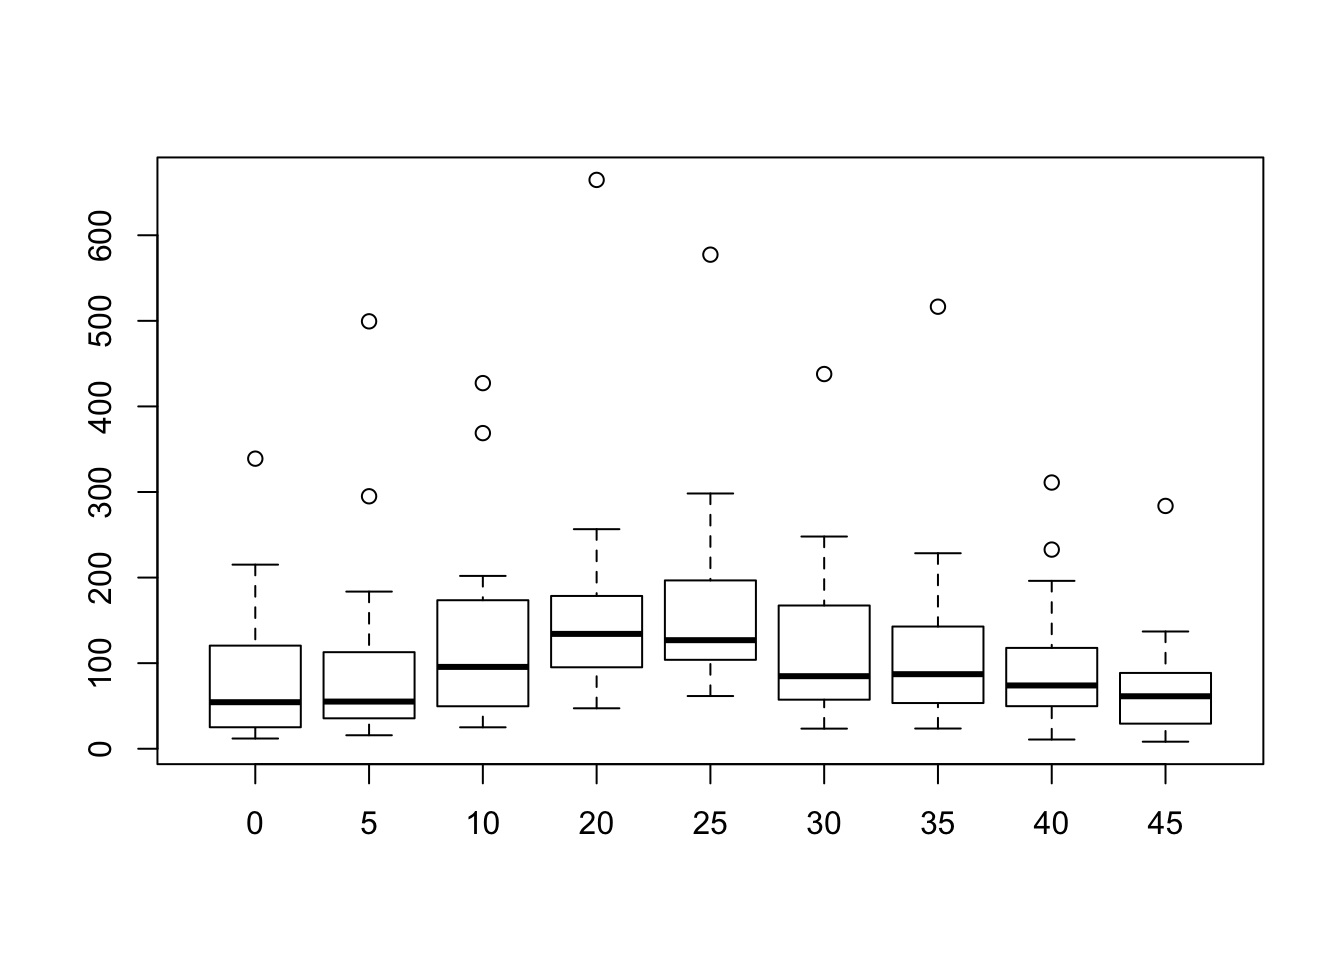
\includegraphics{Zhang_HW2_files/figure-latex/unnamed-chunk-3-1.pdf}

\begin{Shaded}
\begin{Highlighting}[]
\KeywordTok{ggplot}\NormalTok{(CDI, }\KeywordTok{aes}\NormalTok{(Hosp_beds,Physicians)) }\OperatorTok{+}
\StringTok{  }\KeywordTok{geom_point}\NormalTok{(}\DataTypeTok{alpha =} \FloatTok{.1}\NormalTok{, }\DataTypeTok{col =} \StringTok{"blue"}\NormalTok{) }\OperatorTok{+}
\StringTok{  }\KeywordTok{geom_smooth}\NormalTok{(}\KeywordTok{aes}\NormalTok{(}\DataTypeTok{color =} \StringTok{"red"}\NormalTok{),}\DataTypeTok{method =} \StringTok{"lm"}\NormalTok{, }\DataTypeTok{se =} \OtherTok{FALSE}\NormalTok{, }\DataTypeTok{size =} \FloatTok{.3}\NormalTok{) }\OperatorTok{+}\StringTok{ }
\StringTok{  }\KeywordTok{theme_bw}\NormalTok{()}
\end{Highlighting}
\end{Shaded}

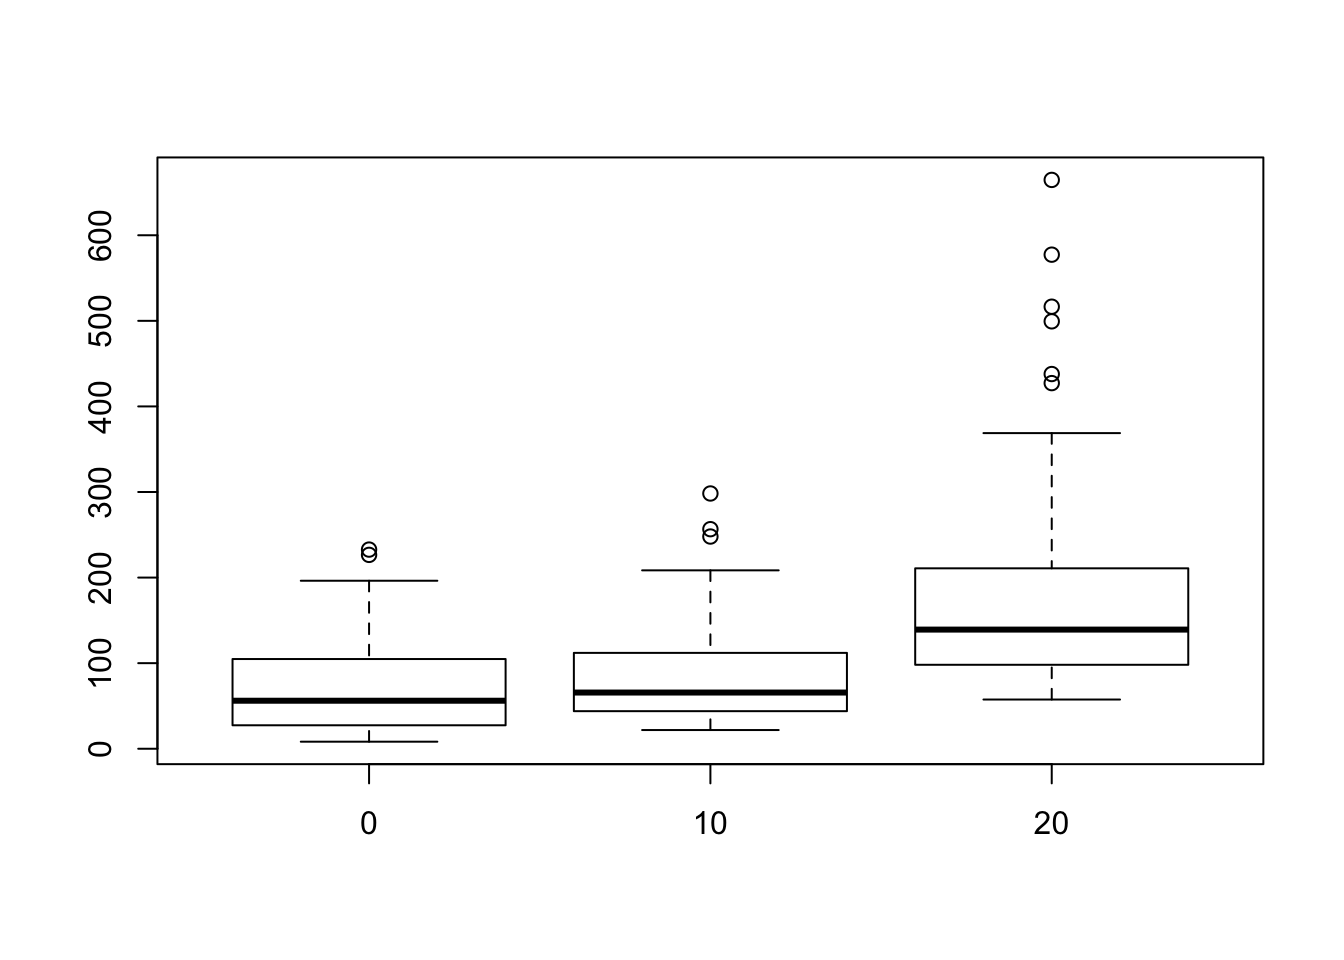
\includegraphics{Zhang_HW2_files/figure-latex/unnamed-chunk-3-2.pdf}

\begin{Shaded}
\begin{Highlighting}[]
\KeywordTok{ggplot}\NormalTok{(CDI, }\KeywordTok{aes}\NormalTok{(Hosp_beds,Physicians)) }\OperatorTok{+}
\StringTok{  }\KeywordTok{geom_point}\NormalTok{(}\DataTypeTok{alpha =} \FloatTok{.1}\NormalTok{, }\DataTypeTok{col =} \StringTok{"blue"}\NormalTok{) }\OperatorTok{+}
\StringTok{  }\KeywordTok{geom_smooth}\NormalTok{(}\KeywordTok{aes}\NormalTok{(}\DataTypeTok{color =} \StringTok{"red"}\NormalTok{), }\DataTypeTok{se =} \OtherTok{FALSE}\NormalTok{, }\DataTypeTok{size =} \FloatTok{.3}\NormalTok{) }\OperatorTok{+}
\StringTok{  }\KeywordTok{theme_bw}\NormalTok{()}
\end{Highlighting}
\end{Shaded}

\begin{verbatim}
## `geom_smooth()` using method = 'loess' and formula 'y ~ x'
\end{verbatim}

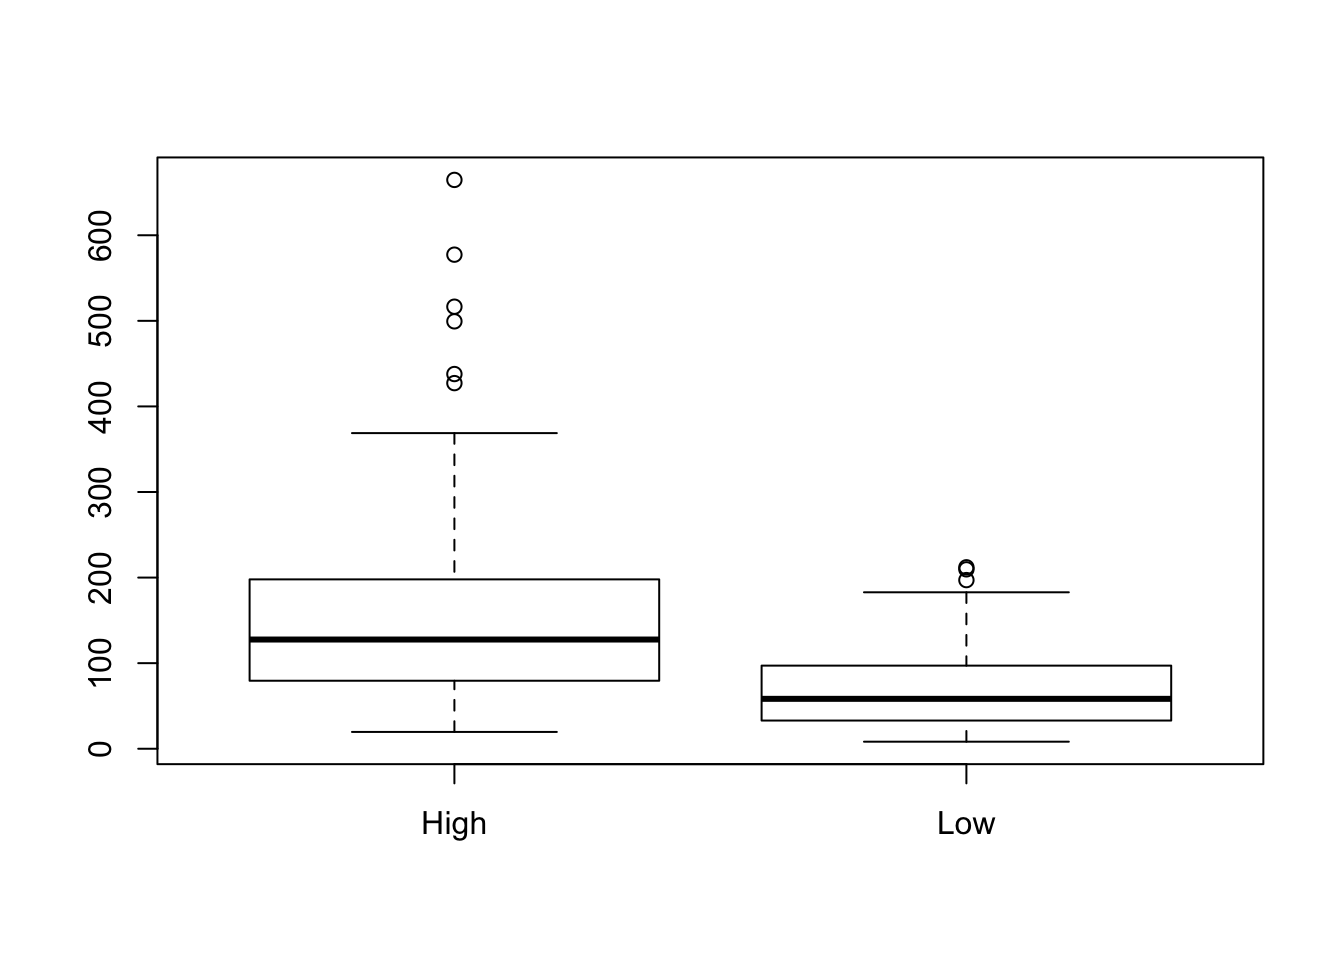
\includegraphics{Zhang_HW2_files/figure-latex/unnamed-chunk-3-3.pdf}

\begin{Shaded}
\begin{Highlighting}[]
\KeywordTok{ggplot}\NormalTok{(CDI, }\KeywordTok{aes}\NormalTok{(PersonalInc,Physicians)) }\OperatorTok{+}
\StringTok{  }\KeywordTok{geom_point}\NormalTok{(}\DataTypeTok{alpha =} \FloatTok{.1}\NormalTok{, }\DataTypeTok{col =} \StringTok{"purple"}\NormalTok{) }\OperatorTok{+}
\StringTok{  }\KeywordTok{geom_smooth}\NormalTok{(}\KeywordTok{aes}\NormalTok{(}\DataTypeTok{color =} \StringTok{"red"}\NormalTok{),}\DataTypeTok{method =} \StringTok{"lm"}\NormalTok{, }\DataTypeTok{se =} \OtherTok{FALSE}\NormalTok{, }\DataTypeTok{size =} \FloatTok{.3}\NormalTok{) }\OperatorTok{+}\StringTok{ }
\StringTok{  }\KeywordTok{theme_bw}\NormalTok{()}
\end{Highlighting}
\end{Shaded}

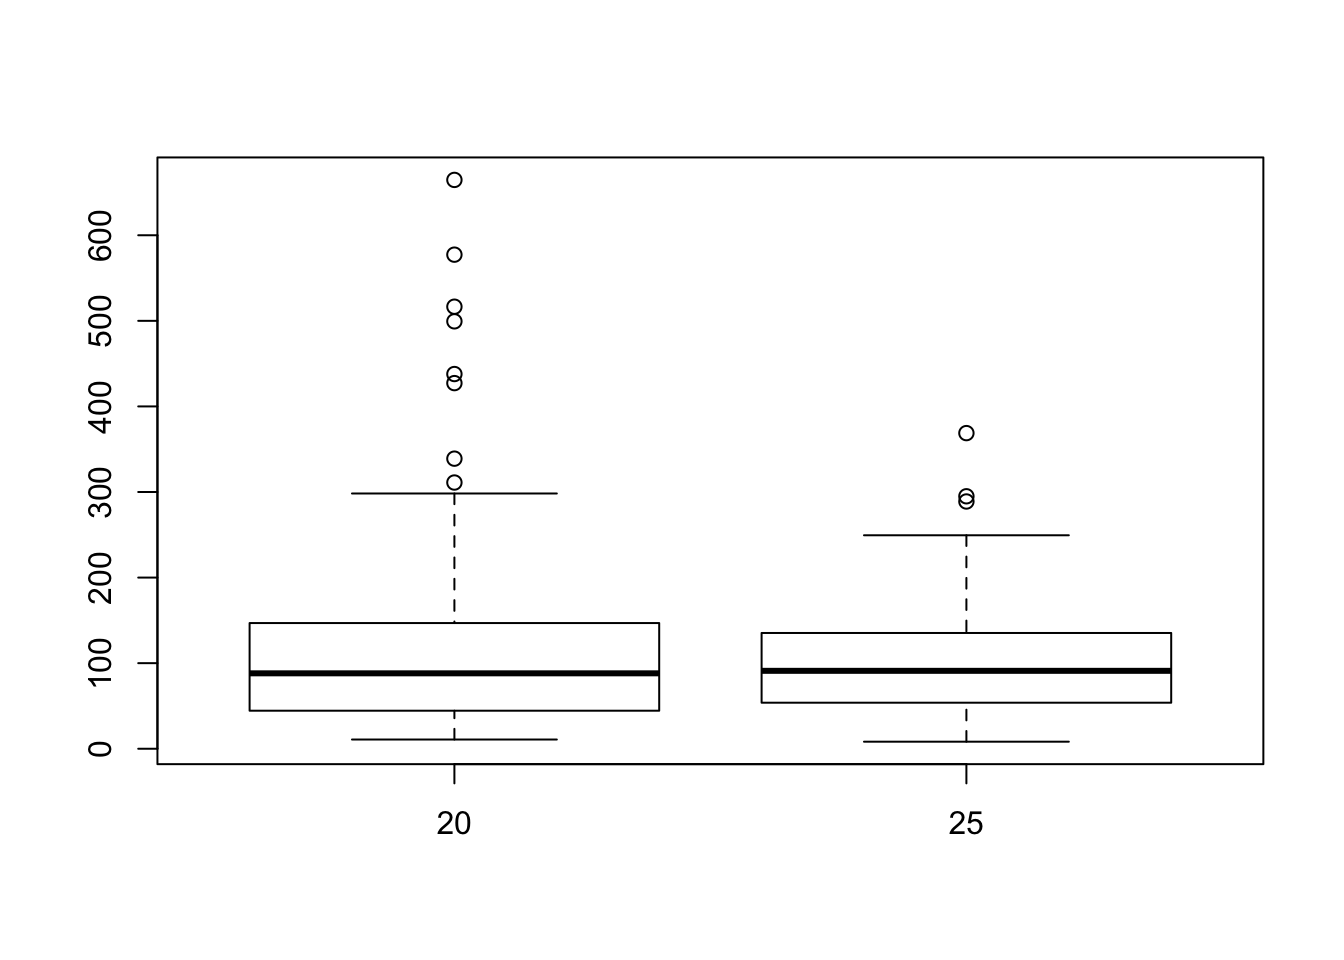
\includegraphics{Zhang_HW2_files/figure-latex/unnamed-chunk-3-4.pdf}

\hypertarget{model-based-on-all-three-predictor-variables-for-fun}{%
\section{Model based on all three predictor variables for
fun:}\label{model-based-on-all-three-predictor-variables-for-fun}}

\begin{Shaded}
\begin{Highlighting}[]
\NormalTok{mod1}\FloatTok{.43}\NormalTok{ =}\StringTok{ }\KeywordTok{lm}\NormalTok{(Physicians }\OperatorTok{~}\StringTok{ }\NormalTok{Pop}\OperatorTok{+}\NormalTok{Hosp_beds}\OperatorTok{+}\NormalTok{PersonalInc, }\DataTypeTok{data =}\NormalTok{ CDI); }\KeywordTok{summary}\NormalTok{(mod1}\FloatTok{.43}\NormalTok{)}
\end{Highlighting}
\end{Shaded}

\begin{verbatim}
## 
## Call:
## lm(formula = Physicians ~ Pop + Hosp_beds + PersonalInc, data = CDI)
## 
## Residuals:
##      Min       1Q   Median       3Q      Max 
## -1931.75  -118.96    -4.76    88.95  2230.98 
## 
## Coefficients:
##               Estimate Std. Error t value Pr(>|t|)    
## (Intercept) -8.910e+01  2.198e+01  -4.054 5.95e-05 ***
## Pop         -1.832e-03  2.116e-04  -8.661  < 2e-16 ***
## Hosp_beds    4.866e-01  2.092e-02  23.263  < 2e-16 ***
## PersonalInc  1.382e-01  8.773e-03  15.754  < 2e-16 ***
## ---
## Signif. codes:  0 '***' 0.001 '**' 0.01 '*' 0.05 '.' 0.1 ' ' 1
## 
## Residual standard error: 379.8 on 436 degrees of freedom
## Multiple R-squared:  0.9553, Adjusted R-squared:  0.955 
## F-statistic:  3104 on 3 and 436 DF,  p-value: < 2.2e-16
\end{verbatim}

\hypertarget{a-number-of-physicians-regressed-on-the-three-predictor-variables-estimated-regression-functions}{%
\subsection{a) Number of physicians regressed on the three predictor
variables; estimated regression
functions:}\label{a-number-of-physicians-regressed-on-the-three-predictor-variables-estimated-regression-functions}}

\begin{Shaded}
\begin{Highlighting}[]
\NormalTok{mod1}\FloatTok{.43}\NormalTok{_pop =}\StringTok{ }\KeywordTok{lm}\NormalTok{(Physicians }\OperatorTok{~}\StringTok{ }\NormalTok{Pop, }\DataTypeTok{data =}\NormalTok{ CDI); }\KeywordTok{summary}\NormalTok{(mod1}\FloatTok{.43}\NormalTok{_pop)}
\end{Highlighting}
\end{Shaded}

\begin{verbatim}
## 
## Call:
## lm(formula = Physicians ~ Pop, data = CDI)
## 
## Residuals:
##     Min      1Q  Median      3Q     Max 
## -1969.4  -209.2   -88.0    27.9  3928.7 
## 
## Coefficients:
##               Estimate Std. Error t value Pr(>|t|)    
## (Intercept) -1.106e+02  3.475e+01  -3.184  0.00156 ** 
## Pop          2.795e-03  4.837e-05  57.793  < 2e-16 ***
## ---
## Signif. codes:  0 '***' 0.001 '**' 0.01 '*' 0.05 '.' 0.1 ' ' 1
## 
## Residual standard error: 610.1 on 438 degrees of freedom
## Multiple R-squared:  0.8841, Adjusted R-squared:  0.8838 
## F-statistic:  3340 on 1 and 438 DF,  p-value: < 2.2e-16
\end{verbatim}

\begin{Shaded}
\begin{Highlighting}[]
\NormalTok{mod1}\FloatTok{.43}\NormalTok{_beds =}\StringTok{ }\KeywordTok{lm}\NormalTok{(Physicians }\OperatorTok{~}\StringTok{ }\NormalTok{Hosp_beds, }\DataTypeTok{data =}\NormalTok{ CDI); }\KeywordTok{summary}\NormalTok{(mod1}\FloatTok{.43}\NormalTok{_beds)}
\end{Highlighting}
\end{Shaded}

\begin{verbatim}
## 
## Call:
## lm(formula = Physicians ~ Hosp_beds, data = CDI)
## 
## Residuals:
##     Min      1Q  Median      3Q     Max 
## -3133.2  -216.8   -32.0    96.2  3611.1 
## 
## Coefficients:
##              Estimate Std. Error t value Pr(>|t|)    
## (Intercept) -95.93218   31.49396  -3.046  0.00246 ** 
## Hosp_beds     0.74312    0.01161  63.995  < 2e-16 ***
## ---
## Signif. codes:  0 '***' 0.001 '**' 0.01 '*' 0.05 '.' 0.1 ' ' 1
## 
## Residual standard error: 556.9 on 438 degrees of freedom
## Multiple R-squared:  0.9034, Adjusted R-squared:  0.9032 
## F-statistic:  4095 on 1 and 438 DF,  p-value: < 2.2e-16
\end{verbatim}

\begin{Shaded}
\begin{Highlighting}[]
\NormalTok{mod1}\FloatTok{.43}\NormalTok{_inc =}\StringTok{ }\KeywordTok{lm}\NormalTok{(Physicians }\OperatorTok{~}\StringTok{ }\NormalTok{PersonalInc, }\DataTypeTok{data =}\NormalTok{ CDI); }\KeywordTok{summary}\NormalTok{(mod1}\FloatTok{.43}\NormalTok{_inc)}
\end{Highlighting}
\end{Shaded}

\begin{verbatim}
## 
## Call:
## lm(formula = Physicians ~ PersonalInc, data = CDI)
## 
## Residuals:
##     Min      1Q  Median      3Q     Max 
## -1926.6  -194.5   -66.6    44.2  3819.0 
## 
## Coefficients:
##              Estimate Std. Error t value Pr(>|t|)    
## (Intercept) -48.39485   31.83333   -1.52    0.129    
## PersonalInc   0.13170    0.00211   62.41   <2e-16 ***
## ---
## Signif. codes:  0 '***' 0.001 '**' 0.01 '*' 0.05 '.' 0.1 ' ' 1
## 
## Residual standard error: 569.7 on 438 degrees of freedom
## Multiple R-squared:  0.8989, Adjusted R-squared:  0.8987 
## F-statistic:  3895 on 1 and 438 DF,  p-value: < 2.2e-16
\end{verbatim}

\hypertarget{b-plots-of-the-estimated-regression-functions-with-their-data}{%
\subsection{b) Plots of the estimated regression functions with their
data:}\label{b-plots-of-the-estimated-regression-functions-with-their-data}}

\hypertarget{regressed-on-population}{%
\section{Regressed on population:}\label{regressed-on-population}}

\begin{Shaded}
\begin{Highlighting}[]
\KeywordTok{plot}\NormalTok{(CDI}\OperatorTok{$}\NormalTok{Pop,CDI}\OperatorTok{$}\NormalTok{Physicians, }\DataTypeTok{pch =} \DecValTok{16}\NormalTok{, }\DataTypeTok{cex =} \FloatTok{.2}\NormalTok{, }\DataTypeTok{col =} \StringTok{"red"}\NormalTok{,}
     \DataTypeTok{main =} \StringTok{"Physicians regressed on population"}\NormalTok{,}
     \DataTypeTok{xlab =} \StringTok{"Population"}\NormalTok{, }\DataTypeTok{ylab =} \StringTok{"Number of Physicians"}\NormalTok{)}
\KeywordTok{abline}\NormalTok{(mod1}\FloatTok{.43}\NormalTok{_pop, }\DataTypeTok{col =} \StringTok{"green"}\NormalTok{)}
\end{Highlighting}
\end{Shaded}

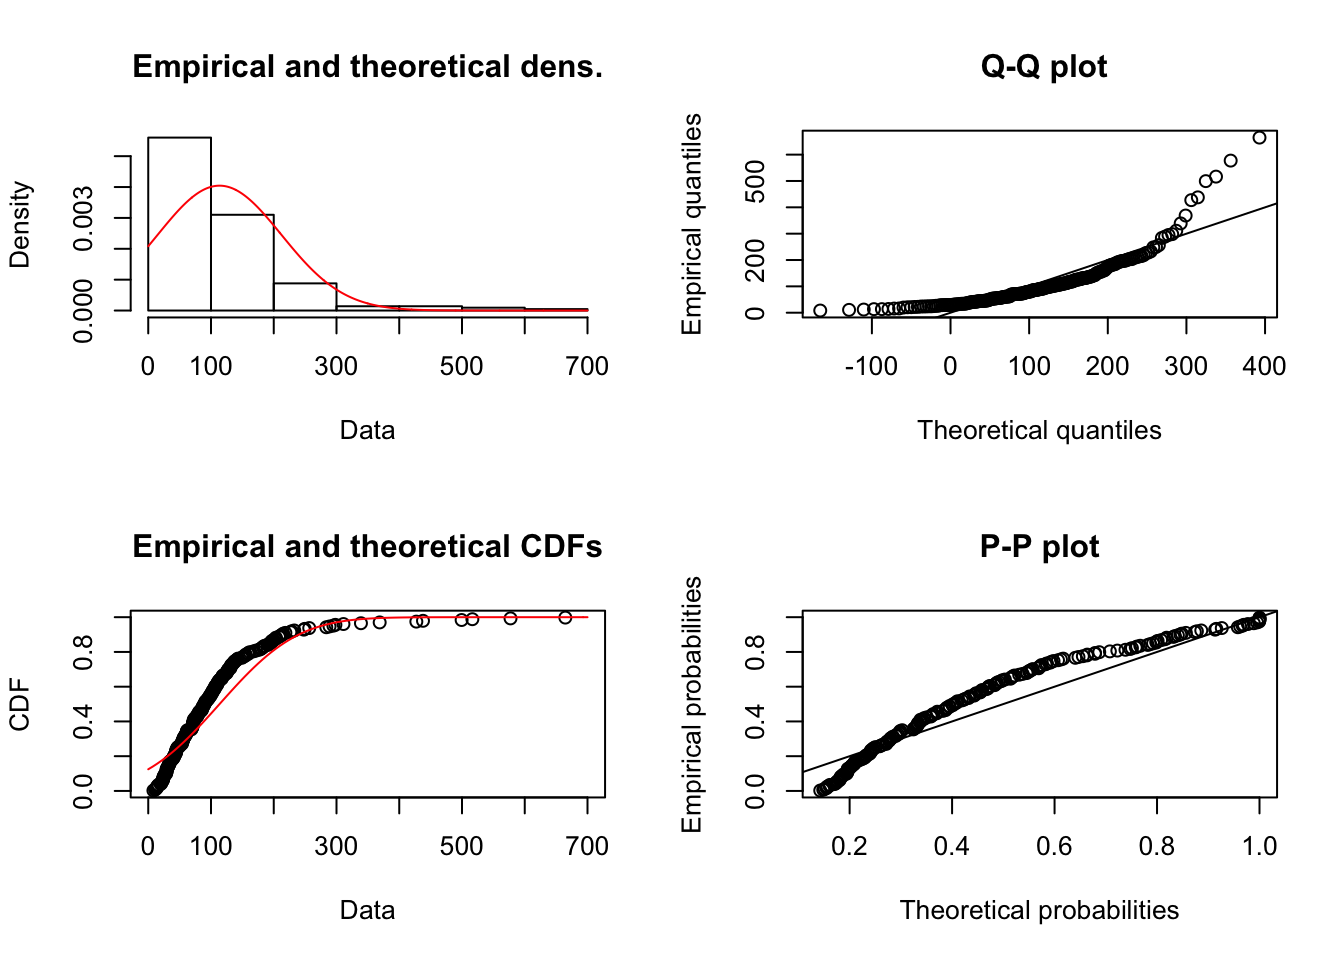
\includegraphics{Zhang_HW2_files/figure-latex/unnamed-chunk-6-1.pdf}

\hypertarget{regressed-on-hospital-beds}{%
\section{Regressed on hospital beds:}\label{regressed-on-hospital-beds}}

\begin{Shaded}
\begin{Highlighting}[]
\KeywordTok{plot}\NormalTok{(CDI}\OperatorTok{$}\NormalTok{Hosp_beds,CDI}\OperatorTok{$}\NormalTok{Physicians, }\DataTypeTok{pch =} \DecValTok{16}\NormalTok{, }\DataTypeTok{cex =} \FloatTok{.2}\NormalTok{, }\DataTypeTok{col =} \StringTok{"red"}\NormalTok{,}
     \DataTypeTok{main =} \StringTok{"Physicians regressed on hospital beds"}\NormalTok{,}
     \DataTypeTok{xlab =} \StringTok{"Hospital beds"}\NormalTok{, }\DataTypeTok{ylab =} \StringTok{"Number of Physicians"}\NormalTok{)}
\KeywordTok{abline}\NormalTok{(mod1}\FloatTok{.43}\NormalTok{_beds, }\DataTypeTok{col =} \StringTok{"green"}\NormalTok{)}
\end{Highlighting}
\end{Shaded}

\includegraphics{Zhang_HW2_files/figure-latex/unnamed-chunk-7-1.pdf}

\hypertarget{a-linear-model-doesnt-appear-to-be-the-best-fit-for-hospital-beds.-it-looks-like-it-might-be-non-linear.}{%
\section{A linear model doesn't appear to be the best fit for hospital
beds. It looks like it might be
non-linear.}\label{a-linear-model-doesnt-appear-to-be-the-best-fit-for-hospital-beds.-it-looks-like-it-might-be-non-linear.}}

\hypertarget{regressed-on-personal-income}{%
\section{Regressed on personal
income:}\label{regressed-on-personal-income}}

\begin{Shaded}
\begin{Highlighting}[]
\KeywordTok{plot}\NormalTok{(CDI}\OperatorTok{$}\NormalTok{PersonalInc,CDI}\OperatorTok{$}\NormalTok{Physicians, }\DataTypeTok{pch =} \DecValTok{16}\NormalTok{, }\DataTypeTok{cex =} \FloatTok{.2}\NormalTok{, }\DataTypeTok{col =} \StringTok{"red"}\NormalTok{,}
     \DataTypeTok{main =} \StringTok{"Physicians regressed on personal income"}\NormalTok{,}
     \DataTypeTok{xlab =} \StringTok{"Personal Income"}\NormalTok{, }\DataTypeTok{ylab =} \StringTok{"Number of Physicians"}\NormalTok{)}
\KeywordTok{abline}\NormalTok{(mod1}\FloatTok{.43}\NormalTok{_inc, }\DataTypeTok{col =} \StringTok{"green"}\NormalTok{)}
\end{Highlighting}
\end{Shaded}

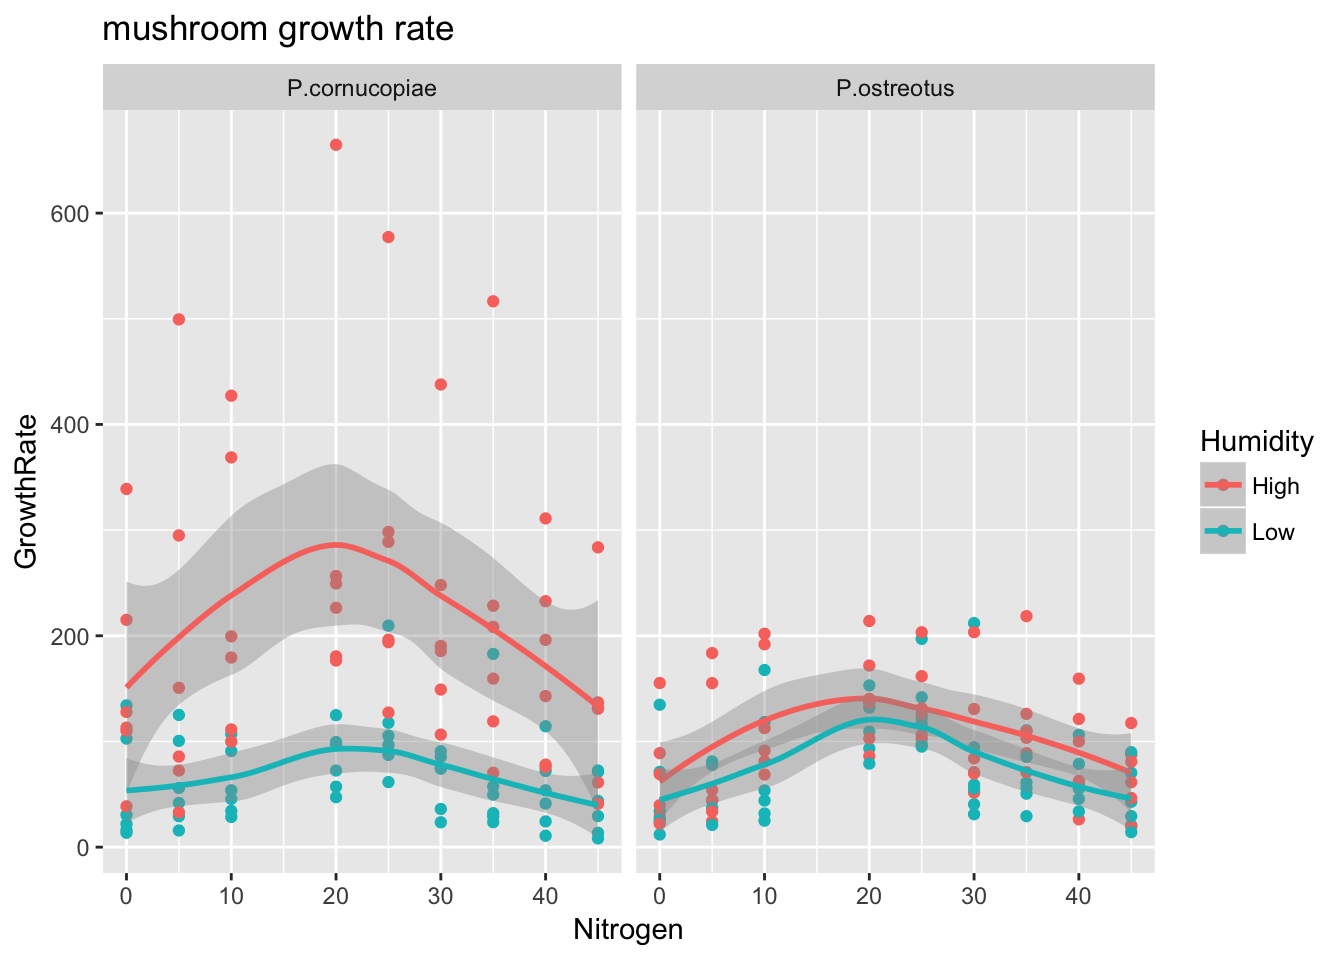
\includegraphics{Zhang_HW2_files/figure-latex/unnamed-chunk-8-1.pdf}

\hypertarget{c-mse-for-each-of-the-predictor-variables}{%
\subsection{c) MSE for each of the predictor
variables:}\label{c-mse-for-each-of-the-predictor-variables}}

\begin{Shaded}
\begin{Highlighting}[]
\NormalTok{msePop =}\StringTok{ }\KeywordTok{mean}\NormalTok{(mod1}\FloatTok{.43}\NormalTok{_pop}\OperatorTok{$}\NormalTok{residuals}\OperatorTok{^}\DecValTok{2}\NormalTok{); msePop}
\end{Highlighting}
\end{Shaded}

\begin{verbatim}
## [1] 370511.7
\end{verbatim}

\begin{Shaded}
\begin{Highlighting}[]
\NormalTok{mseBeds =}\StringTok{ }\KeywordTok{mean}\NormalTok{(mod1}\FloatTok{.43}\NormalTok{_beds}\OperatorTok{$}\NormalTok{residuals}\OperatorTok{^}\DecValTok{2}\NormalTok{); mseBeds}
\end{Highlighting}
\end{Shaded}

\begin{verbatim}
## [1] 308781.9
\end{verbatim}

\begin{Shaded}
\begin{Highlighting}[]
\NormalTok{mseInc =}\StringTok{ }\KeywordTok{mean}\NormalTok{(mod1}\FloatTok{.43}\NormalTok{_inc}\OperatorTok{$}\NormalTok{residuals}\OperatorTok{^}\DecValTok{2}\NormalTok{); mseInc}
\end{Highlighting}
\end{Shaded}

\begin{verbatim}
## [1] 323064.2
\end{verbatim}

\hypertarget{section-1}{%
\subsubsection{2.2}\label{section-1}}

\hypertarget{in-a-test-of-the-alternatives-ho-beta1-0-versus-ha-beta1-0-an-analyst-concluded-ho.-does-this-mean-there-is-no-linear-association-between-x-and-y}{%
\section{In a test of the alternatives Ho: beta1 ≤ 0 versus Ha: beta1
\textgreater{} 0, an analyst concluded Ho. Does this mean there is no
linear association between X and
Y?}\label{in-a-test-of-the-alternatives-ho-beta1-0-versus-ha-beta1-0-an-analyst-concluded-ho.-does-this-mean-there-is-no-linear-association-between-x-and-y}}

\hypertarget{i-would-say-that-it-doesnt-mean-the-association-is-not-linear-or-that-there-is-no-linear-association.-it-could-be-that-the-association-is-linear-and-negative-i.e.that-x-and-y-are-negatively-correlated-in-a-linear-way.}{%
\section{I would say that it doesn't mean the association is not linear
or that there is no linear association. It could be that the association
is linear and negative (i.e.~that X and Y are negatively correlated in a
linear
way).}\label{i-would-say-that-it-doesnt-mean-the-association-is-not-linear-or-that-there-is-no-linear-association.-it-could-be-that-the-association-is-linear-and-negative-i.e.that-x-and-y-are-negatively-correlated-in-a-linear-way.}}

\hypertarget{section-2}{%
\subsubsection{2.17}\label{section-2}}

\hypertarget{the-alpha-level-used-was-greater-than-.033.-if-the-alpha-had-been-.01-then-the-appropriate-conclusion-would-have-been-ho.}{%
\section{The alpha level used was greater than .033. If the alpha had
been .01, then the appropriate conclusion would have been
Ho.}\label{the-alpha-level-used-was-greater-than-.033.-if-the-alpha-had-been-.01-then-the-appropriate-conclusion-would-have-been-ho.}}

\hypertarget{section-3}{%
\subsubsection{2.62}\label{section-3}}

\hypertarget{reviewing-again-the-models-from-1.43}{%
\section{Reviewing again the models from
1.43:}\label{reviewing-again-the-models-from-1.43}}

\begin{Shaded}
\begin{Highlighting}[]
\NormalTok{mod1}\FloatTok{.43}\NormalTok{_pop =}\StringTok{ }\KeywordTok{lm}\NormalTok{(Physicians }\OperatorTok{~}\StringTok{ }\NormalTok{Pop, }\DataTypeTok{data =}\NormalTok{ CDI); }\KeywordTok{summary}\NormalTok{(mod1}\FloatTok{.43}\NormalTok{_pop)}
\end{Highlighting}
\end{Shaded}

\begin{verbatim}
## 
## Call:
## lm(formula = Physicians ~ Pop, data = CDI)
## 
## Residuals:
##     Min      1Q  Median      3Q     Max 
## -1969.4  -209.2   -88.0    27.9  3928.7 
## 
## Coefficients:
##               Estimate Std. Error t value Pr(>|t|)    
## (Intercept) -1.106e+02  3.475e+01  -3.184  0.00156 ** 
## Pop          2.795e-03  4.837e-05  57.793  < 2e-16 ***
## ---
## Signif. codes:  0 '***' 0.001 '**' 0.01 '*' 0.05 '.' 0.1 ' ' 1
## 
## Residual standard error: 610.1 on 438 degrees of freedom
## Multiple R-squared:  0.8841, Adjusted R-squared:  0.8838 
## F-statistic:  3340 on 1 and 438 DF,  p-value: < 2.2e-16
\end{verbatim}

\begin{Shaded}
\begin{Highlighting}[]
\NormalTok{mod1}\FloatTok{.43}\NormalTok{_beds =}\StringTok{ }\KeywordTok{lm}\NormalTok{(Physicians }\OperatorTok{~}\StringTok{ }\NormalTok{Hosp_beds, }\DataTypeTok{data =}\NormalTok{ CDI); }\KeywordTok{summary}\NormalTok{(mod1}\FloatTok{.43}\NormalTok{_beds)}
\end{Highlighting}
\end{Shaded}

\begin{verbatim}
## 
## Call:
## lm(formula = Physicians ~ Hosp_beds, data = CDI)
## 
## Residuals:
##     Min      1Q  Median      3Q     Max 
## -3133.2  -216.8   -32.0    96.2  3611.1 
## 
## Coefficients:
##              Estimate Std. Error t value Pr(>|t|)    
## (Intercept) -95.93218   31.49396  -3.046  0.00246 ** 
## Hosp_beds     0.74312    0.01161  63.995  < 2e-16 ***
## ---
## Signif. codes:  0 '***' 0.001 '**' 0.01 '*' 0.05 '.' 0.1 ' ' 1
## 
## Residual standard error: 556.9 on 438 degrees of freedom
## Multiple R-squared:  0.9034, Adjusted R-squared:  0.9032 
## F-statistic:  4095 on 1 and 438 DF,  p-value: < 2.2e-16
\end{verbatim}

\begin{Shaded}
\begin{Highlighting}[]
\NormalTok{mod1}\FloatTok{.43}\NormalTok{_inc =}\StringTok{ }\KeywordTok{lm}\NormalTok{(Physicians }\OperatorTok{~}\StringTok{ }\NormalTok{PersonalInc, }\DataTypeTok{data =}\NormalTok{ CDI); }\KeywordTok{summary}\NormalTok{(mod1}\FloatTok{.43}\NormalTok{_inc)}
\end{Highlighting}
\end{Shaded}

\begin{verbatim}
## 
## Call:
## lm(formula = Physicians ~ PersonalInc, data = CDI)
## 
## Residuals:
##     Min      1Q  Median      3Q     Max 
## -1926.6  -194.5   -66.6    44.2  3819.0 
## 
## Coefficients:
##              Estimate Std. Error t value Pr(>|t|)    
## (Intercept) -48.39485   31.83333   -1.52    0.129    
## PersonalInc   0.13170    0.00211   62.41   <2e-16 ***
## ---
## Signif. codes:  0 '***' 0.001 '**' 0.01 '*' 0.05 '.' 0.1 ' ' 1
## 
## Residual standard error: 569.7 on 438 degrees of freedom
## Multiple R-squared:  0.8989, Adjusted R-squared:  0.8987 
## F-statistic:  3895 on 1 and 438 DF,  p-value: < 2.2e-16
\end{verbatim}

\hypertarget{population-r2-.8838}{%
\section{Population R\^{}2 : .8838}\label{population-r2-.8838}}

\hypertarget{hospital-beds-r2-.9032}{%
\section{Hospital beds R\^{}2 : .9032}\label{hospital-beds-r2-.9032}}

\hypertarget{hospital-beds-accounts-for-the-largest-reduction-in-the-variability-in-the-number-of-active-physicians}{%
\paragraph{Hospital beds accounts for the largest reduction in the
variability in the number of active
physicians}\label{hospital-beds-accounts-for-the-largest-reduction-in-the-variability-in-the-number-of-active-physicians}}

\hypertarget{personal-income-r2-.8987}{%
\section{Personal income R\^{}2 :
.8987}\label{personal-income-r2-.8987}}


\end{document}
